%% (√(200) - 10) + (20 - √(200))
\documentclass[tikz]{standalone}
\usepackage{amsmath,amsfonts,amssymb,mathrsfs,tikz,fancyhdr}
\usepackage{fontspec}
\usepackage{unicode-math}
\usepackage{tikz}
\usepackage{tkz-euclide}
\usepackage{bidi}

\begin{document}

% \setmainfont[Script=Arabic,Mapping=arabicdigits]{Amiri}
% \setmathfont{XITS Math}

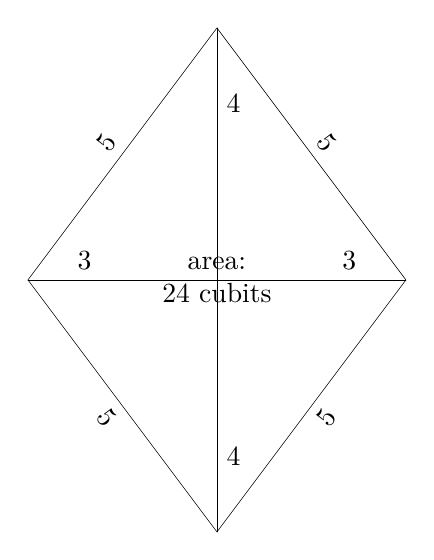
\begin{tikzpicture}[scale=0.8]
  % Define vertices based on half-diagonals (4,0) and (0,3)
  \tkzDefPoints{3/0/A, 0/4/B, -3/0/C, 0/-4/D, 0/0/O}
  % Draw polygon and diagonals
  \tkzDrawPolygon(A,B,C,D)
  \tkzDrawSegments(A,C B,D)

  \path (D)--(B) node[midway,align=center]
  {area:\\ 24 cubits};

  \path (A)--(B) node[midway,sloped,above] {\RL{5}};
  \path (B)--(C) node[midway,sloped,above] {\RL{5}};
  \path (C)--(D) node[midway,sloped,below] {\RL{5}};
  \path (D)--(A) node[midway,sloped,below] {\RL{5}};

  \path (O)--(A) node[pos=0.7,above] {\RL{3}};
  \path (O)--(C) node[pos=0.7,above] {\RL{3}};
  \path (O)--(B) node[pos=0.7,right] {\RL{4}};
  \path (O)--(D) node[pos=0.7,right] {\RL{4}};

\end{tikzpicture}

\end{document}